%%%%%%%%%%%%%%%%%%%%%%%%%%%%%%%%%%%%%%%%%%%%%%%%%%%%
% LECTURE 23: THERMAL RADIATION
%%%%%%%%%%%%%%%%%%%%%%%%%%%%%%%%%%%%%%%%%%%%%%%%%%%%
\section*{Thermal Radiation}
\addcontentsline{toc}{section}{Thermal Radiation}

%%%%%%%%%%%%%%%%%%%%%%%%%%%%%%%%%%%%%%%%%%%%%%%%%%%%
\subsection*{Introduction to Thermal Radiation}
\addcontentsline{toc}{subsection}{Introduction to Thermal Radiation}
%%%%%%%%%%%%%%%%%%%%%%%%%%%%%%%%%%%%%%%%%%%%%%%%%%%%

This lecture begins the third part of the heat transfer course, focusing on thermal radiation. The final exam will cover comprehensive material including all heat transfer modes, and may involve identifying which modes are dominant in different scenarios. We will spend approximately four weeks on radiation, with the last lecture reserved for review and comprehensive problems.
%%%%%%%%%%%%%%%%%%%%%%%%%%%%%%%%%%%%%%%%%%%%%%%%%%%%
\subsubsection*{Recap of Simple Radiation Model}
\addcontentsline{toc}{subsubsection}{Recap of Simple Radiation Model}
%%%%%%%%%%%%%%%%%%%%%%%%%%%%%%%%%%%%%%%%%%%%%%%%%%%%
In previous sections, we used a simplified radiation model for isothermal surfaces in isothermal enclosures. The net heat flux between the surface and its surroundings is given by:

\[
    q'' = \varepsilon \sigma (T_{\text{sur}}^4 - T_{\text{surrounding}}^4)
\]

Where:
\begin{itemize}
    \item $\varepsilon$ is the emissivity (dimensionless, between 0 and 1)
    \item $\sigma$ is the Stefan-Boltzmann constant: $5.67 \times 10^{-8}$ W/m$^2$K$^4$
    \item $T_{\text{surface}}$ and $T_{\text{surrounding}}$ must be in Kelvin
\end{itemize}

However, this formula is limited in its applications. It cannot handle:
\begin{itemize}
    \item Surfaces with temperature gradients
    \item Environments with non-uniform surrounding temperatures
    \item Complex geometric interactions between surfaces
\end{itemize}

This section of the course will develop a more comprehensive understanding of radiation heat transfer, starting with the physics of the process, defining relevant terminology, and building protocols to calculate radiation exchange between multiple surfaces.

%%%%%%%%%%%%%%%%%%%%%%%%%%%%%%%%%%%%%%%%%%%%%%%%%%%%
\subsection*{Physical Origin of Thermal Radiation}
\addcontentsline{toc}{subsection}{Physical Origin of Thermal Radiation}
%%%%%%%%%%%%%%%%%%%%%%%%%%%%%%%%%%%%%%%%%%%%%%%%%%%%
\subsubsection*{Fundamental Concepts}
\addcontentsline{toc}{subsubsection}{Fundamental Concepts}
%%%%%%%%%%%%%%%%%%%%%%%%%%%%%%%%%%%%%%%%%%%%%%%%%%%%
Several key concepts underpin our understanding of thermal radiation:

\begin{enumerate}
    \item \textbf{Vacuum as a material medium}: For radiation calculations, vacuum itself must be considered as a medium with specific material properties that allow electromagnetic waves to propagate.
    
    \item \textbf{Universal emission}: All matter with a finite absolute temperature emits thermal radiation in the form of Electromagnetic Waves (EMW).
    
    \item \textbf{Absorption requirement}: If materials emit radiation, they must also be capable of absorbing radiation; otherwise, thermodynamic laws would be violated.
    
    \item \textbf{Speed of propagation}: Electromagnetic waves travel at the speed of light ($c \approx 3 \times 10^8$ m/s in vacuum), which is essentially instantaneous for most heat transfer applications.
    
    \item \textbf{Wave characteristics}: Electromagnetic waves can be described by either wavelength ($\lambda$) or frequency ($f$), with the relationship $c = \lambda f$.
\end{enumerate}

\subsubsection*{Dipole Oscillation Mechanism}
\addcontentsline{toc}{subsubsection}{Dipole Oscillation Mechanism}

Thermal radiation originates at the atomic level through oscillating electric dipoles:

\begin{itemize}
    \item An electric dipole consists of a positive and negative charge separated by a small distance
    \item When a dipole oscillates, it generates an oscillating electromagnetic field that propagates outward
    \item The strength and frequency of the electromagnetic wave are determined by the strength and frequency of the dipole's oscillation
    \item In real materials, dipole oscillations are driven by internal thermal energy
    \item Higher temperatures correspond to more energetic oscillations, producing more intense radiation
\end{itemize}
%
So
\begin{itemize}
    \item EMWs can be seen as oscillating EM fields driven by displacement of charges.
    \item Outband EMW are determined by strength and frequency of oscillations.
\end{itemize}
%
Thermal energy causes random motion of atoms and molecules, which drives the oscillation of dipoles. This randomness follows the statistics of thermodynamics and forms the basis for blackbody radiation theory.
\[  
    \begin{aligned}
        & \text{Thermal Energy} \rightarrow \text{EMW rich in freq/$\lambda $}
        \\
        &\text{Higher T (more internal Energy $U$)} \rightarrow \text{ stronger radiation} 
    \end{aligned}
\]

\subsubsection*{Spectrum of Electromagnetic Waves}
\addcontentsline{toc}{subsubsection}{Spectrum of Electromagnetic Waves}

If we were to oscillate a dipole from very low frequencies up to very high frequencies ($\nu:0 \to \infty$), we would generate radiation across the electromagnetic spectrum:

\begin{itemize}
    \item At very low frequencies: invisible radiation
    \item At approximately 430 THz: visible red light
    \item Increasing frequency: orange, yellow, green, blue, violet
    \item At very high frequencies: invisible again (ultraviolet)
\end{itemize}

Energy increases with frequency, which is why blue/violet light (higher frequency) carries more energy per photon than red light (lower frequency).

Thermal radiation spans a significant portion of the electromagnetic spectrum, with different wavelength regions categorized as:

\begin{itemize}
    \item Ultraviolet (UV): Below 0.4 $\mu$m
    \item Visible: 0.4-0.7 $\mu$m
    \item Near Infrared: 0.7-2 $\mu$m
    \item Mid Infrared: 2-5 $\mu$m
    \item Far Infrared: 5-100 $\mu$m
    \item Microwave: 100 $\mu$m to centimeters
    \item Radio: Centimeters and longer
\end{itemize}

For thermal engineering applications, we are primarily concerned with wavelengths from approximately 0.1 $\mu$m to 100 $\mu$m, depending on the temperature range of interest.
%
\begin{figure}[H]
    \centering
    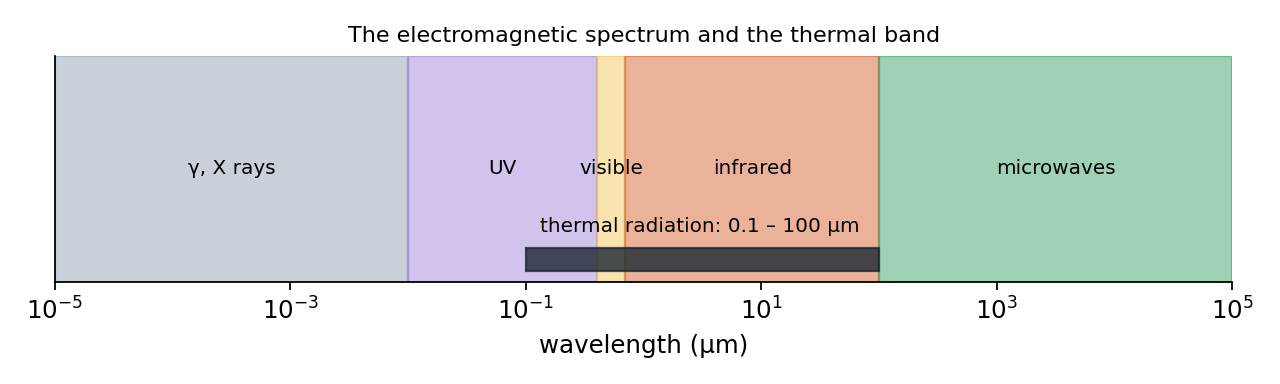
\includegraphics[width=0.8\linewidth]{pics/Electromagnetic radiation spectrum.png}
    \caption{Electromagnetic radiation spectrum}
\end{figure}
%
\subsubsection*{Material Interaction with Radiation}
\addcontentsline{toc}{subsubsection}{Material Interaction with Radiation}

Real materials can be conceptualized as collections of dipoles. Their interaction with radiation depends on several factors:

\begin{itemize}
    \item \textbf{Emission depth}: In most solid materials, only dipoles near the surface (within a "skin depth") can emit radiation that reaches the outside world.
    
    \item \textbf{Material opacity}: Materials that strongly absorb/emit radiation are considered opaque. For metals, the skin depth is typically 10-100 nanometers. For dielectrics like glass or water, it ranges from micrometers to millimeters.
    
    \item \textbf{Transmission}: If the material thickness is less than the skin depth, some radiation can transmit through, making the material semi-transparent.
    
    \item \textbf{Scattering}: Heterogeneous materials like fog or particulate suspensions can scatter radiation, making analysis more complex.
\end{itemize}

In this course, we will focus primarily on opaque materials, touch upon transparent materials, and only briefly introduce semi-transparent materials and scattering phenomena.

\subsubsection*{Time Scales and Physics}
\addcontentsline{toc}{subsubsection}{Time Scales and Physics}

Thermal radiation involves extremely fast processes:
\begin{itemize}
    \item Photon emission/absorption: Femtoseconds ($10^{-15}$ s)
    \item Heat diffusion from skin layer: Picoseconds to nanoseconds ($10^{-12}$ to $10^{-9}$ s)
\end{itemize}

This rapid timescale means we typically don't need to model absorption skin layers separately, as energy is quickly distributed in the material.

Another important characteristic of thermal radiation is the low photon density. Each photon essentially acts independently, without interacting with other photons. This makes the process linear and allows for simple superposition of radiation effects.

%%%%%%%%%%%%%%%%%%%%%%%%%%%%%%%%%%%%%%%%%%%%%%%%%%%%
\subsection*{Characterization of Thermal Emission}
\addcontentsline{toc}{subsection}{Characterization of Thermal Emission}
%%%%%%%%%%%%%%%%%%%%%%%%%%%%%%%%%%%%%%%%%%%%%%%%%%%%

\subsubsection*{Spectral and Directional Characteristics}
\addcontentsline{toc}{subsubsection}{Spectral and Directional Characteristics}

Thermal radiation from real surfaces varies in two important ways:

\begin{enumerate}
    \item \textbf{Spectral Distribution}:Thermal radiation emitted by a surface encompasses a range of wavelengths. As shown in Figure \ref{fig:spectral}, the magnitude of the radiation varies with wavelength, and the term spectral is used to refer to the nature of this dependence. As we will find, both the magnitude of the radiation at any wavelength and the spectral distribution vary with the nature and temperature of the emitting surface.
    
    \item \textbf{Directional Distribution}: The radiation intensity varies with the angle from the surface. This is constrained by thermodynamics, which prevents perfect collimation of thermal radiation. It can be measured by moving a detector around the surface.
\end{enumerate}

These distributions help us characterize how different materials radiate energy.
%
\begin{figure}[H]
    \centering
    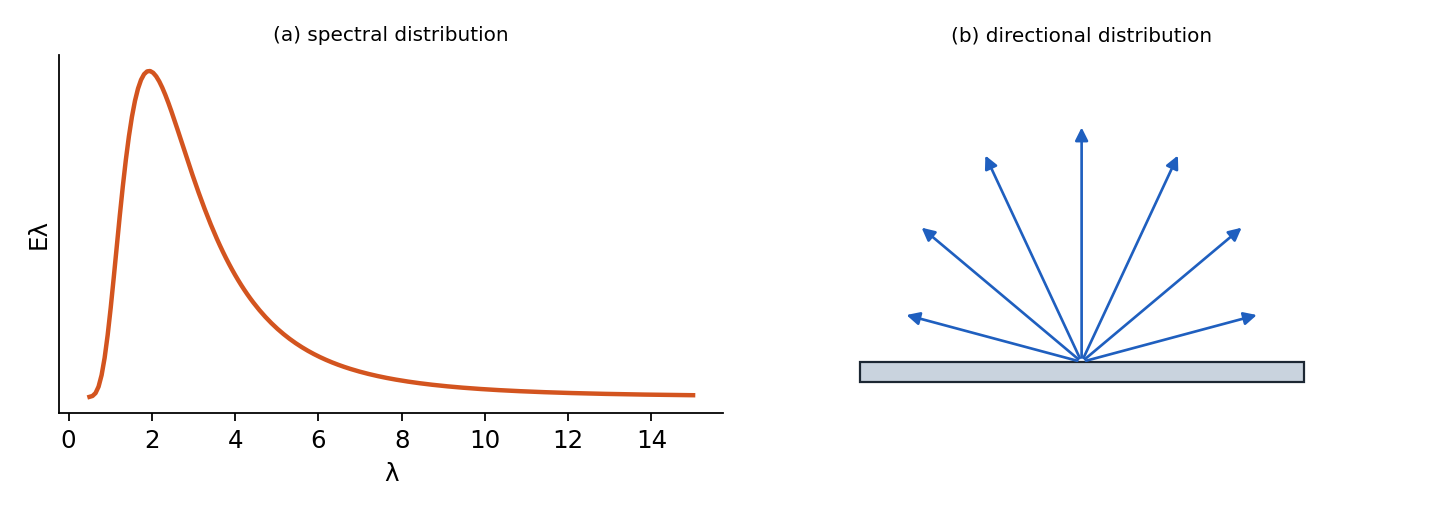
\includegraphics[width=0.7\linewidth]{pics/spectral_and_directional.png}
    \caption{Radiation emitted by a surface. (a) Spectral distribution. (b) Directional distribution.}
    \label{fig:spectral}
\end{figure}
%
\subsubsection*{Surface Types}
\addcontentsline{toc}{subsubsection}{Surface Types}

Real surfaces can generally be classified into two categories based on their directional emission patterns:

\begin{itemize}
    \item \textbf{Diffuse}: Surfaces where the power density (intensity) is uniform regardless of viewing angle. White paper appears equally bright from different angles because it's approximately diffuse.
    
    \item \textbf{Non-diffuse}: Surfaces where radiation intensity varies with direction. Glossy surfaces like glass or polished metal exhibit preferential reflection in certain directions.
\end{itemize}

%%%%%%%%%%%%%%%%%%%%%%%%%%%%%%%%%%%%%%%%%%%%%%%%%%%%
\subsection*{Mathematical Foundations for Radiation}
\addcontentsline{toc}{subsection}{Mathematical Foundations for Radiation}
%%%%%%%%%%%%%%%%%%%%%%%%%%%%%%%%%%%%%%%%%%%%%%%%%%%%

\subsubsection*{Solid Angle Concept}
\addcontentsline{toc}{subsubsection}{Solid Angle Concept}

To describe radiation in three-dimensional space, we use the concept of solid angles:

\begin{itemize}
    \item \textbf{2D angle}: $d\alpha = \frac{dl}{r}$  [rad]
    \item \textbf{3D solid angle}: $d\omega = \frac{dA_n}{r^2}$ [sr] (steradian)
\end{itemize}

For reference:
\begin{itemize}
    \item 2D half space: $\frac{\pi r}{r} = \pi$ [rad], full space: $2\pi$ [rad]
    \item 3D half space: $2\pi$ [sr], full space: $4\pi$ [sr]
\end{itemize}
%
%
\begin{figure}[H]
    \centering
    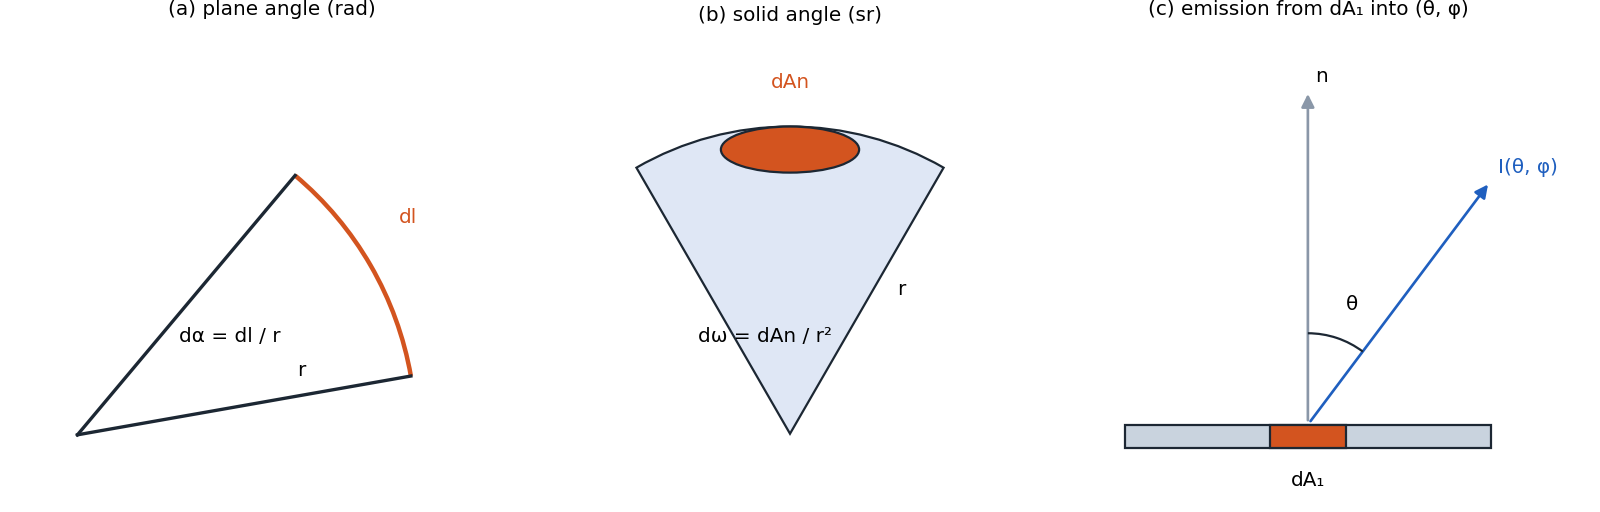
\includegraphics[width=0.7\linewidth]{pics/Mathematical_definitions_angles.png}
    \caption{Mathematical definitions. (a) Plane angle. (b) Solid angle. (c) Emission of radiation from a differential area $d A_1$ into a solid angle $d \omega$ subtended by $d A_n$ at a point on $d A_1$. (d) The spherical coordinate system.}
\end{figure}
%
Note that the unit of the solid
angle is the steradian (sr), analogous to radians for plane angles.

\subsubsection*{3D Solid Angle in Spherical Coordinates}
\addcontentsline{toc}{subsubsection}{3D Solid Angle in Spherical Coordinates}

In spherical coordinates, the solid angle differential is:
\[
d\omega = \sin\theta \, d\theta \, d\phi
\]
%
\begin{figure}[H]
    \centering
    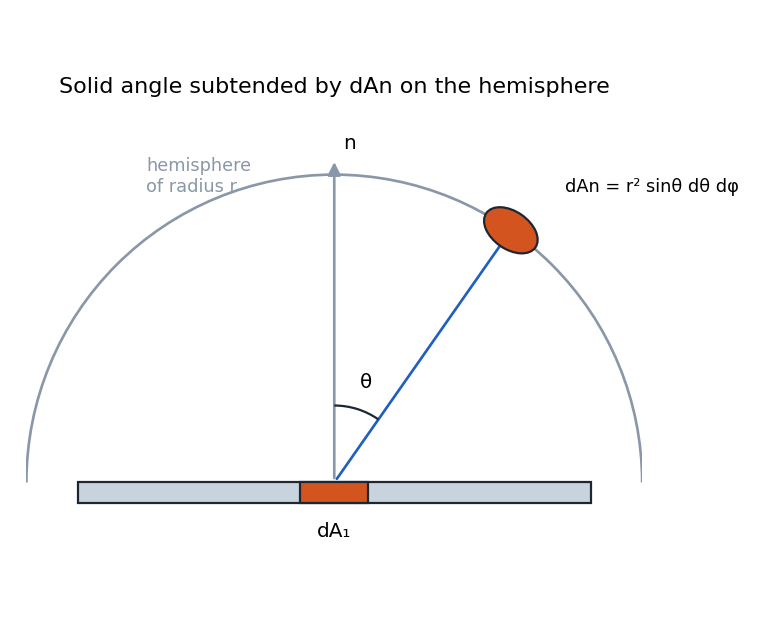
\includegraphics[width=0.7\linewidth]{pics/solid_angle_sphere.png}
    \caption{The solid angle subtended by $d A_n$ at a point on $d A_1$ in the spherical coordinate system.}
\end{figure}

%%%%%%%%%%%%%%%%%%%%%%%%%%%%%%%%%%%%%%%%%%%%%%%%%%%%
\subsubsection*{Summary}
\addcontentsline{toc}{subsubsection}{Summary}
%%%%%%%%%%%%%%%%%%%%%%%%%%%%%%%%%%%%%%%%%%%%%%%%%%%%

\begin{itemize}
    \item Radiation is characterized by wavelength
    \item Radiation processes happen extremely fast, requiring temporal approximations
    \item Emission and absorption are complementary processes with thermodynamic restrictions
\end{itemize}

%LECTURE 24 (ANOTHER VERSION)
% %%%%%%%%%%%%%%%%%%%%%%%%%%%%%%%%%%%%%%%%%%%%%%%%%%%%
% \subsection*{Radiation Heat Fluxes and Radiative Properties}
% \addcontentsline{toc}{subsection}{Radiation Heat Fluxes and Radiative Properties}
% %%%%%%%%%%%%%%%%%%%%%%%%%%%%%%%%%%%%%%%%%%%%%%%%%%%%

% \subsubsection*{Energy Interaction with Surfaces}
% \addcontentsline{toc}{subsubsection}{Energy Interaction with Surfaces}

% When radiation strikes a surface, the energy can be divided into three components:

% \textbf{For semi-transparent media:}
% \[
% G = G_{\text{ref}} + G_{\text{abs}} + G_{\text{tr}}
% \]

% Where:
% \begin{itemize}
%     \item $G$ is the incident radiation (irradiation)
%     \item $G_{\text{ref}}$ is the reflected portion
%     \item $G_{\text{abs}}$ is the absorbed portion
%     \item $G_{\text{tr}}$ is the transmitted portion
% \end{itemize}

% \textbf{For opaque media:}
% \[
% G = G_{\text{ref}} + G_{\text{abs}}
% \]
% with no transmission term.

% \subsubsection*{Radiosity Concept}
% \addcontentsline{toc}{subsubsection}{Radiosity Concept}

% Radiosity ($J$) represents the total radiative energy leaving a surface:
% \[
% J = G_{\text{ref}} + E
% \]

% Where $E$ is the emissive power of the surface, given by:
% \[
% E = \varepsilon \sigma T_s^4
% \]

% The net heat flux leaving the surface is:
% \[
% q''_{\text{rad}} = J - G
% \]

% \subsubsection*{Radiative Properties}
% \addcontentsline{toc}{subsubsection}{Radiative Properties}

% We define several radiative properties to characterize surface behavior:

% \textbf{1. Absorptivity:}

% Spectral, directional absorptivity:
% \[
% \alpha_{\lambda,\theta}(\lambda,\theta,\phi) = \frac{I_{\lambda,i,\text{abs}}(\lambda,\theta,\phi)}{I_{\lambda,i}(\lambda,\theta,\phi)}
% \]

% Spectral, hemispherical absorptivity:
% \[
% \alpha_{\lambda} = \frac{G_{\lambda,\text{abs}}(\lambda)}{G_{\lambda}(\lambda)}
% \]

% Total, hemispherical absorptivity:
% \[
% \alpha = \frac{G_{\text{abs}}}{G}
% \]

% \textbf{2. Reflectivity:}

% Spectral, directional reflectivity:
% \[
% \rho_{\lambda,\theta}(\lambda,\theta,\phi) = \frac{I_{\lambda,i,\text{ref}}(\lambda,\theta,\phi)}{I_{\lambda,i}(\lambda,\theta,\phi)}
% \]

% Spectral, hemispherical reflectivity:
% \[
% \rho_{\lambda} = \frac{G_{\lambda,\text{ref}}(\lambda)}{G_{\lambda}(\lambda)}
% \]

% Total, hemispherical reflectivity:
% \[
% \rho = \frac{G_{\text{ref}}}{G}
% \]

% \textbf{3. Transmissivity:}

% Spectral, directional transmissivity:
% \[
% \tau_{\lambda,\theta}(\lambda,\theta,\phi) = \frac{I_{\lambda,i,\text{tr}}(\lambda,\theta,\phi)}{I_{\lambda,i}(\lambda,\theta,\phi)}
% \]

% Spectral, hemispherical transmissivity:
% \[
% \tau_{\lambda} = \frac{G_{\lambda,\text{tr}}(\lambda)}{G_{\lambda}(\lambda)}
% \]

% Total, hemispherical transmissivity:
% \[
% \tau = \frac{G_{\text{tr}}}{G}
% \]

% \subsubsection*{Conservation Relationships}
% \addcontentsline{toc}{subsubsection}{Conservation Relationships}

% For all radiative interactions, the conservation of energy requires:

% \textbf{For semi-transparent media:}
% \[
% \rho_{\lambda} + \alpha_{\lambda} + \tau_{\lambda} = 1 \quad \text{(spectral)}
% \]
% \[
% \rho + \alpha + \tau = 1 \quad \text{(total)}
% \]

% \textbf{For opaque media:}
% \[
% \rho_{\lambda} + \alpha_{\lambda} = 1 \quad \text{(spectral)}
% \]
% \[
% \rho + \alpha = 1 \quad \text{(total)}
% \]

% \subsubsection*{Radiation Intensity Measures}
% \addcontentsline{toc}{subsubsection}{Radiation Intensity Measures}

% Radiation intensity is defined by heat flux per wavelength per solid angle:

% \[
% I_{\lambda,e}(\lambda,\theta,\phi) = \frac{dq}{dA_1 \cdot \cos\theta \cdot d\omega \cdot d\lambda} \left[\frac{\text{W}}{\text{m}^2 \cdot \text{sr} \cdot \mu\text{m}}\right]
% \]

% \textbf{Important note:} Intensity is not a function of distance for collimated beams in non-absorbing media.

% Irradiation intensity is similarly defined:

% \[
% I_{\lambda,i}(\lambda,\theta,\phi) = \frac{dq_{\text{incident}}}{dA_1 \cos\theta \cdot d\omega\cdot d\lambda} \left[\frac{\text{W}}{\text{m}^2 \cdot \text{sr} \cdot \mu\text{m}}\right]
% \]

% \subsubsection*{General Terms for Radiation}
% \addcontentsline{toc}{subsubsection}{General Terms for Radiation}

% Several key flux terms are used in radiation calculations:

% \textbf{1. Spectral hemispherical flux:}

% For emission:
% \[
% E_{\lambda}(\lambda) = q''_{\lambda}(\lambda) = \int_0^{2\pi} \int_0^{\pi/2} I_{\lambda,e}(\lambda,\theta,\phi) \sin\theta \cos\theta \, d\theta \, d\phi \left[\frac{\text{W}}{\text{m}^2 \cdot \mu\text{m}}\right]
% \]

% For irradiation:
% \[
% G_{\lambda}(\lambda) = \int_0^{2\pi} \int_0^{\pi/2} I_{\lambda,i}(\lambda,\theta,\phi) \sin\theta \cos\theta \, d\theta \, d\phi \left[\frac{\text{W}}{\text{m}^2 \cdot \mu\text{m}}\right]
% \]

% \textbf{2. Total heat flux:}

% For emission:
% \[
% E = q'' = \int_0^{\infty} E_{\lambda}(\lambda) \, d\lambda \quad \text{or} \quad \int_0^{\infty} E_{\lambda}(\lambda) \, d\lambda \left[\frac{\text{W}}{\text{m}^2}\right]
% \]

% For irradiation:
% \[
% G = \int_0^{\infty} G_{\lambda}(\lambda) \, d\lambda \left[\frac{\text{W}}{\text{m}^2}\right]
% \]

% \subsubsection*{Diffuse Radiation}
% \addcontentsline{toc}{subsubsection}{Diffuse Radiation}

% For diffuse surfaces, the radiation intensity is independent of direction:

% For emission:
% \[
% I_{\lambda,e}(\lambda,\theta,\phi) = I_{\lambda,e}(\lambda)
% \]

% For irradiation:
% \[
% I_{\lambda,i}(\lambda,\theta,\phi) = I_{\lambda,i}(\lambda)
% \]

% The total emission of a diffuse surface simplifies to:
% \[
% E = \int_0^{\infty} E_{\lambda} \, d\lambda = \int_0^{\infty} \left(\int_0^{2\pi} \int_0^{\pi/2} I_{\lambda,e}(\lambda) \sin\theta \cos\theta \, d\theta \, d\phi \right) \, d\lambda = \pi I_e \left[\frac{\text{W}}{\text{m}^2}\right]
% \]

% Similarly, for diffuse irradiation:
% \[
% G = \pi I_i \left[\frac{\text{W}}{\text{m}^2}\right]
% \]

% \subsubsection*{Total Radiosity}
% \addcontentsline{toc}{subsubsection}{Total Radiosity}

% For a diffuse surface in diffuse irradiation:
% \[
% J = \pi I_e + \rho \pi I_i = \pi I_e + \pi I_r = \pi I_{e+r}
% \]

% Where $I_r = \rho I_i$ is the reflected intensity.

% %%%%%%%%%%%%%%%%%%%%%%%%%%%%%%%%%%%%%%%%%%%%%%%%%%%%
% \subsection*{Radiative Quantities Summary}
% \addcontentsline{toc}{subsection}{Radiative Quantities Summary}
% %%%%%%%%%%%%%%%%%%%%%%%%%%%%%%%%%%%%%%%%%%%%%%%%%%%%

% \begin{itemize}
%     \item \textbf{Three types of radiative quantities:}
%     \begin{itemize}
%         \item $E$ — Emitted radiation from a surface
%         \item $G$ — Incident radiation onto a surface
%         \item $J$ — Radiosity (total radiation leaving a surface)
%     \end{itemize}
    
%     \item \textbf{Defined physical quantities:}
%     \begin{itemize}
%         \item Intensity: $I_{\lambda,e}$, $I_{\lambda,i}$, $I_{\lambda,e+r}$ $\left[\frac{\text{W}}{\text{m}^2 \cdot \text{sr} \cdot \mu\text{m}}\right]$
%         \item Spectral fluxes: $E_{\lambda}$, $G_{\lambda}$, $J_{\lambda}$ $\left[\frac{\text{W}}{\text{m}^2 \cdot \mu\text{m}}\right]$
%         \item Total fluxes: $E$, $G$, $J$ $\left[\frac{\text{W}}{\text{m}^2}\right]$
%     \end{itemize}
    
%     \item \textbf{Terms used in radiation analysis:}
%     \begin{itemize}
%         \item Spectral, hemispherical, total
%         \item Diffuse surface (emission, reflection)
%         \item Diffuse emission, diffuse irradiation
%     \end{itemize}
% \end{itemize}

% \textbf{Special notes:}
% \begin{itemize}
%     \item Intensities are defined based on normal area (cosine term in definitions)
%     \item Fluxes are defined based on actual surface area (cosine term in integrations)
%     \item In this class, we usually assume diffuse emission, diffuse reflection, and diffuse irradiation, with or without spectral distributions
% \end{itemize}

% %%%%%%%%%%%%%%%%%%%%%%%%%%%%%%%%%%%%%%%%%%%%%%%%%%%%
% \subsection*{Blackbody Radiation}
% \addcontentsline{toc}{subsection}{Blackbody Radiation}
% %%%%%%%%%%%%%%%%%%%%%%%%%%%%%%%%%%%%%%%%%%%%%%%%%%%%

% \subsubsection*{Blackbody Concept}
% \addcontentsline{toc}{subsubsection}{Blackbody Concept}

% A blackbody is an important conceptual reference for radiation analysis. It has the following properties:

% \begin{itemize}
%     \item Absorbs all incident radiation (for all $\lambda$, $\theta$, $\phi$)
%     \item Emits the maximum possible energy at a given temperature and wavelength (still a function of $T$ and $\lambda$)
%     \item Exhibits diffuse emission characteristics
% \end{itemize}

% Perfect absorbers and perfect emitters don't exist in reality, but they serve as useful theoretical references. A small hole in a large cavity approximates a blackbody.

% \subsubsection*{Planck Distribution}
% \addcontentsline{toc}{subsubsection}{Planck Distribution}

% The spectral emissive power of a blackbody is described by Planck's distribution:

% \[
% E_{\lambda,b}(\lambda,T) = \pi I_{\lambda,b}(\lambda,T) = \frac{C_1}{\lambda^5[\exp(C_2/\lambda T)-1]}
% \]

% Where:
% \begin{align}
% C_1 &= 2\pi h c_0^2 = 3.742 \times 10^8 \frac{\text{W} \cdot \mu\text{m}^4}{\text{m}^2} \\
% C_2 &= \frac{h c_0}{k} = 1.439 \times 10^4 \, \mu\text{m} \cdot \text{K} \\
% h &= 6.626 \times 10^{-34} \, \text{J} \cdot \text{s} \quad \text{(Planck's constant)} \\
% k &= 1.381 \times 10^{-23} \, \text{J}/\text{K} \quad \text{(Boltzmann's constant)} \\
% c_0 &= 2.998 \times 10^8 \, \text{m}/\text{s} \quad \text{(speed of light in vacuum)} \\
% T &= \text{absolute temperature [K]}
% \end{align}

% The spectral distribution varies with temperature, with the peak of emission shifting to shorter wavelengths as temperature increases.

% \subsubsection*{Stefan-Boltzmann Law}
% \addcontentsline{toc}{subsubsection}{Stefan-Boltzmann Law}

% The total emissive power from a blackbody is obtained by integrating the Planck distribution:

% \[
% E_b = \int_0^{\infty} E_{\lambda,b} \, d\lambda = \sigma T^4 \quad \text{($\varepsilon=1$ for blackbody)}
% \]

% Where $\sigma = 5.67 \times 10^{-8}$ W/m$^2$K$^4$ is the Stefan-Boltzmann constant.

% \subsubsection*{Wien's Displacement Law}
% \addcontentsline{toc}{subsubsection}{Wien's Displacement Law}

% The wavelength of maximum emission for a blackbody is inversely proportional to its temperature:

% \[
%     \lambda_{\max} \cdot T = 2897.8 \, \mu\text{m} \cdot \text{K}
% \]

% This explains why:
% \begin{itemize}
%     \item Sun ($\approx$ 5800 K): Peak emission in visible spectrum ($\approx$ 0.5 $\mu$m)
%     \item Light bulb ($\approx$ 2900 K): Peak in near infrared ($\approx$ 1.0 $\mu$m)
%     \item Room temperature objects ($\approx$300 K): Peak in far infrared ($\approx$ 10 $\mu$m)
% \end{itemize}

% \subsubsection*{Band Emission}
% \addcontentsline{toc}{subsubsection}{Band Emission}

% For simplifying calculations, we often consider the fraction of blackbody emission within a specific wavelength range:

% \[
% F_{(0 \rightarrow \lambda)} = \frac{\int_0^{\lambda} E_{\lambda,b} \, d\lambda}{\int_0^{\infty} E_{\lambda,b} \, d\lambda} = \int_0^{\lambda T} \frac{E_{\lambda,b}}{\sigma T^5} \, d(\lambda T) = f(\lambda T)
% \]

% This fraction depends only on the product $\lambda T$, and values are tabulated for convenience.

% %%%%%%%%%%%%%%%%%%%%%%%%%%%%%%%%%%%%%%%%%%%%%%%%%%%%
% \subsection*{Emission from Real Surfaces}
% \addcontentsline{toc}{subsection}{Emission from Real Surfaces}
% %%%%%%%%%%%%%%%%%%%%%%%%%%%%%%%%%%%%%%%%%%%%%%%%%%%%

% Real surfaces emit less radiation than blackbodies at the same temperature. We use emissivity to quantify this relationship:

% \[
% \text{Emissivity} = \frac{\text{Radiation emitted by real surface}}{\text{Radiation emitted by blackbody at same $T_s$}}
% \]

% \subsubsection*{Types of Emissivity}
% \addcontentsline{toc}{subsubsection}{Types of Emissivity}

% \begin{enumerate}
%     \item \textbf{Spectral, directional emissivity:}
%     \[
%     \varepsilon_{\lambda,\theta}(\lambda,\theta,\phi,T_s) = \frac{I_{\lambda,e}(\lambda,\theta,\phi,T_s)}{I_{\lambda,b}(\lambda,T_s)}
%     \]
    
%     \item \textbf{Total directional emissivity:}
%     \[
%     \varepsilon_{\theta}(\theta,\phi,T_s) = \frac{I_e(\theta,\phi,T_s)}{I_b(T_s)}
%     \]
    
%     \item \textbf{Spectral, hemispherical emissivity:}
%     \[
%     \varepsilon_{\lambda}(\lambda,T_s) = \frac{E_{\lambda}(\lambda,T_s)}{E_{\lambda,b}(\lambda,T_s)}
%     \]
    
%     \item \textbf{Total emissivity:}
%     \[
%     \varepsilon(T_s) = \frac{E(T_s)}{E_b(T_s)}
%     \]
% \end{enumerate}

% \subsubsection*{Important Properties of Emissivity}
% \addcontentsline{toc}{subsubsection}{Important Properties of Emissivity}

% \begin{itemize}
%     \item Metals typically have low emissivity
%     \item Dielectrics (oxidized surfaces) typically have high emissivity
%     \item Emissivity varies with angle - typically constant for small angles, then drops rapidly near 90° for conductors
%     \item In many cases, we can approximate: $\varepsilon \approx \varepsilon_n$ (where $\varepsilon_n$ is emissivity at normal direction, $\theta = 0^\circ \mathrm{C}$)
% \end{itemize}

% %%%%%%%%%%%%%%%%%%%%%%%%%%%%%%%%%%%%%%%%%%%%%%%%%%%%
% \subsection*{Kirchhoff's Law}
% \addcontentsline{toc}{subsection}{Kirchhoff's Law}
% %%%%%%%%%%%%%%%%%%%%%%%%%%%%%%%%%%%%%%%%%%%%%%%%%%%%

% \subsubsection*{Relationship Between Emissivity and Absorptivity}
% \addcontentsline{toc}{subsubsection}{Relationship Between Emissivity and Absorptivity}

% Kirchhoff's law establishes a fundamental relationship between emissivity and absorptivity. Consider a large isothermal enclosure (temperature $T_s$) containing small bodies ($A_1$, $A_2$, $A_3$). These bodies are too small to affect the radiation field.

% Under these conditions:
% \begin{itemize}
%     \item The irradiation is $G = E_b(T_s) = \sigma T_s^4$
%     \item At thermal equilibrium, all surfaces reach the same temperature: $T_1 = T_2 = T_3 = T_s$
% \end{itemize}

% Considering energy balance on body $A_1$:
% \[
% \alpha_1 \cdot G \cdot A_1 - E_1(T_s) \cdot A_1 = 0
% \]

% This yields:
% \[
% \alpha_1 E_b(T_s) = E_1(T_s)
% \]

% Since emissivity is defined as $\varepsilon_1 = \frac{E_1}{E_b}$, we conclude:
% \[
% \varepsilon_1 = \alpha_1, \quad \varepsilon_2 = \alpha_2, \quad \varepsilon_3 = \alpha_3
% \]

% Therefore, at isothermal conditions:
% \[
% \varepsilon = \alpha
% \]

% \subsubsection*{Extension to Spectral and Directional Properties}
% \addcontentsline{toc}{subsubsection}{Extension to Spectral and Directional Properties}

% This equality can be extended to spectral and directional properties:
% \[
% \alpha_{\lambda} = \varepsilon_{\lambda}
% \]
% \[
% \alpha_{\lambda,\theta} = \varepsilon_{\lambda,\theta}
% \]

% These relationships hold true for an object inside a large isothermal enclosure.

% \subsubsection*{Further Extensions of Kirchhoff's Law}
% \addcontentsline{toc}{subsubsection}{Further Extensions of Kirchhoff's Law}

% More generally, Kirchhoff's law can be extended to various conditions:

% \begin{enumerate}
%     \item In its most fundamental form, $\varepsilon_{\lambda,\theta} = \alpha_{\lambda,\theta}$ at any surface temperature (inherent surface property)
    
%     \item If irradiation is diffuse OR the surface is diffuse:
%     \[
%     \varepsilon_{\lambda} = \alpha_{\lambda}
%     \]
    
%     \item If irradiation corresponds to that of a blackbody at the surface temperature, OR if the surface is gray and conditions for (2) hold:
%     \[
%     \varepsilon = \alpha
%     \]
% \end{enumerate}

% The last condition is the most commonly applied in engineering heat transfer calculations, especially for opaque surfaces.

% %%%%%%%%%%%%%%%%%%%%%%%%%%%%%%%%%%%%%%%%%%%%%%%%%%%%
% \subsection*{View Factors for Radiation Exchange}
% \addcontentsline{toc}{subsection}{View Factors for Radiation Exchange}
% %%%%%%%%%%%%%%%%%%%%%%%%%%%%%%%%%%%%%%%%%%%%%%%%%%%%

% To analyze radiation exchange between surfaces, we need to quantify how surfaces "see" each other geometrically. This is done using view factors.

% \subsubsection*{View Factor Definition}
% \addcontentsline{toc}{subsubsection}{View Factor Definition}

% The view factor (also called shape factor or configuration factor) $F_{ij}$ represents the fraction of radiation leaving surface $i$ that directly reaches surface $j$:

% \[
% F_{ij} = \frac{q_{i \rightarrow j}}{q_i}
% \]

% Where:
% \begin{itemize}
%     \item $q_i$ is the total radiation leaving surface $i$ (radiosity × area)
%     \item $q_{i \rightarrow j}$ is the radiation from surface $i$ that falls on surface $j$
% \end{itemize}

% \subsubsection*{View Factor Relations}
% \addcontentsline{toc}{subsubsection}{View Factor Relations}

% View factors have several important properties:

% \begin{enumerate}
%     \item \textbf{Reciprocity relation}: $A_i F_{ij} = A_j F_{ji}$
    
%     This relates view factors between pairs of surfaces based on their areas.
    
%     \item \textbf{Addition rule}: $F_{i \rightarrow (j+k)} = F_{i \rightarrow j} + F_{i \rightarrow k}$
    
%     This allows combining or dividing surfaces to determine view factors.
    
%     \item \textbf{Summation rule}: $\sum_{j=1}^N F_{ij} = 1$ for an enclosure of $N$ surfaces
    
%     All radiation leaving a surface must strike some surface in the enclosure.
    
%     \item \textbf{Self-viewing rule}:
%     \begin{itemize}
%         \item $F_{ii} = 0$ for flat or convex surfaces
%         \item $F_{ii} > 0$ for concave surfaces
%     \end{itemize}
    
%     \item \textbf{Hypothetical/fake surface rule}:
%     \[
%     F_{real \rightarrow another} = \frac{A_{fake}}{A_{real}} F_{fake \rightarrow another}
%     \]
    
%     This helps handle complex geometries by introducing hypothetical surfaces.
% \end{enumerate}

% View factors for common geometries are available in tables and charts in heat transfer references. For example, Table 13.1 provides view factors for two-dimensional configurations, while Table 13.2 covers three-dimensional configurations.

% %%%%%%%%%%%%%%%%%%%%%%%%%%%%%%%%%%%%%%%%%%%%%%%%%%%%
% \subsection*{Radiation Exchange Between Gray-Diffuse Surfaces}
% \addcontentsline{toc}{subsection}{Radiation Exchange Between Gray-Diffuse Surfaces}
% %%%%%%%%%%%%%%%%%%%%%%%%%%%%%%%%%%%%%%%%%%%%%%%%%%%%

% The main difference between gray enclosures and black enclosures is the presence of reflection. In gray enclosures:

% \begin{itemize}
%     \item Surfaces reflect radiation
%     \item Even surfaces that cannot "see" each other directly can exchange energy via reflection
%     \item We assume diffuse, gray, opaque surfaces at uniform temperatures
% \end{itemize}

% \subsubsection*{Radiosity for Gray Surfaces}
% \addcontentsline{toc}{subsubsection}{Radiosity for Gray Surfaces}

% The radiosity for a gray surface can be expressed as:
% \[
% J = E + \rho G = \varepsilon E_b + (1-\varepsilon) G
% \]

% Where:
% \begin{itemize}
%     \item $E$ is the emission from the surface
%     \item $\rho G$ is the reflected portion of irradiation
%     \item $\varepsilon E_b$ is the blackbody emission scaled by emissivity
%     \item $(1-\varepsilon)$ is the reflectivity (using Kirchhoff's law: $\rho = 1 - \alpha = 1 - \varepsilon$)
% \end{itemize}

% \subsubsection*{Net Energy Leaving a Surface}
% \addcontentsline{toc}{subsubsection}{Net Energy Leaving a Surface}

% The net energy leaving a surface is:
% \[
% \frac{q}{A} = J - G = \varepsilon E_b + (1-\varepsilon)G - G = \varepsilon (E_b - G)
% \]

% This can be rearranged to:
% \[
% q = \varepsilon A (E_b - G) = \varepsilon A \left(E_b - \frac{J-\varepsilon E_b}{1-\varepsilon}\right) = \frac{\varepsilon A}{1-\varepsilon}(E_b - J)
% \]

% \subsubsection*{Electrical Circuit Analogy}
% \addcontentsline{toc}{subsubsection}{Electrical Circuit Analogy}

% Radiation heat transfer can be conceptualized using an electrical circuit analogy:

% \begin{itemize}
%     \item Potential difference: $E_b - J$ (analogous to voltage)
%     \item Heat rate: $q$ (analogous to current)
%     \item Resistance: $\frac{1-\varepsilon}{\varepsilon A}$ (surface resistance to radiation)
% \end{itemize}

% This is represented in circuit form as:
% \[
% q = \frac{E_b - J}{\frac{1-\varepsilon}{\varepsilon A}}
% \]

% The surface resistance $\frac{1-\varepsilon}{\varepsilon A}$ represents how easily heat can radiate from a surface, with lower resistance for higher emissivity.

% \subsubsection*{Net Radiation Exchange Between Two Surfaces}
% \addcontentsline{toc}{subsubsection}{Net Radiation Exchange Between Two Surfaces}

% For two surfaces exchanging radiation:
% \[
% q_{12} = J_1 A_1 F_{12} - J_2 A_2 F_{21}
% \]

% Using the reciprocity relation $A_1 F_{12} = A_2 F_{21}$, this simplifies to:
% \[
% q_{12} = \frac{J_1 - J_2}{1/A_1 F_{12}}
% \]

% The term $1/A_1 F_{12}$ represents the "space resistance" between the two surfaces. This resistance depends only on geometry, measuring how easily the surfaces can exchange radiation.

% %%%%%%%%%%%%%%%%%%%%%%%%%%%%%%%%%%%%%%%%%%%%%%%%%%%%
% \subsection*{Radiation Networks}
% \addcontentsline{toc}{subsection}{Radiation Networks}
% %%%%%%%%%%%%%%%%%%%%%%%%%%%%%%%%%%%%%%%%%%%%%%%%%%%%

% Complex radiation problems can be solved using a network approach:

% \begin{enumerate}
%     \item Draw the radiation network with nodes representing surface radiosities ($J_i$)
%     \item Connect nodes with resistances representing:
%     \begin{itemize}
%         \item Surface resistances: $\frac{1-\varepsilon_i}{\varepsilon_i A_i}$
%         \item Space resistances: $\frac{1}{A_i F_{ij}}$
%     \end{itemize}
%     \item Apply energy balance at each node using:
%     \[
%     \frac{E_{bi} - J_i}{(1-\varepsilon_i)/\varepsilon_i A_i} = \sum_{j=1}^{N} \frac{J_i - J_j}{1/A_i F_{ij}}
%     \]
%     \item Solve the resulting system of equations for the unknown radiosities
% \end{enumerate}

% \subsubsection*{Radiation Quantities Between Surfaces}
% \addcontentsline{toc}{subsubsection}{Radiation Quantities Between Surfaces}

% Several important radiation quantities help us analyze heat transfer between surfaces:

% \begin{itemize}
%     \item $q_{i \rightarrow j}$: Rate of radiation that leaves surface $i$ and falls on surface $j$
%     \item $q_{ij}$: Net radiation exchange between surfaces $i$ and $j$ (positive when leaving $i$)
%     \[
%     q_{ij} = q_{i \rightarrow j} - q_{j \rightarrow i}
%     \]
%     \item $q_i$: Total net radiation loss for surface $i$
%     \[
%     q_i = \sum_{j=1}^{N} q_{ij}
%     \]
% \end{itemize}

% Important properties of these quantities:
% \begin{itemize}
%     \item $q_{ij} = -q_{ji}$ (radiation exchange is equal and opposite)
%     \item $q_{i \rightarrow j} \neq q_{j \rightarrow i}$ (gross radiation flows may differ)
%     \item $\sum_{i=1}^{N} q_i = 0$ (conservation of energy for an enclosure)
% \end{itemize}

% %%%%%%%%%%%%%%%%%%%%%%%%%%%%%%%%%%%%%%%%%%%%%%%%%%%%
% \subsection*{Re-Radiating Surfaces}
% \addcontentsline{toc}{subsection}{Re-Radiating Surfaces}
% %%%%%%%%%%%%%%%%%%%%%%%%%%%%%%%%%%%%%%%%%%%%%%%%%%%%

% A re-radiating surface is a special case in radiation heat transfer:
% \begin{itemize}
%     \item Thermally insulated for both conduction and convection
%     \item No net energy exchange with its surroundings
%     \item Simply redistributes incoming radiation
% \end{itemize}

% For a re-radiating surface $R$ with parameters $A_R$, $T_R$, and $\varepsilon_R$:
% \begin{itemize}
%     \item Net heat transfer $q_R = 0$
%     \item Blackbody emissive power $E_{bR} = J_R$ (surface radiosity equals blackbody emission)
% \end{itemize}

% This condition simplifies the radiation network by eliminating the surface resistance for re-radiating surfaces.

% %%%%%%%%%%%%%%%%%%%%%%%%%%%%%%%%%%%%%%%%%%%%%%%%%%%%
% \subsection*{Multi-Mode Heat Transfer}
% \addcontentsline{toc}{subsection}{Multi-Mode Heat Transfer}
% %%%%%%%%%%%%%%%%%%%%%%%%%%%%%%%%%%%%%%%%%%%%%%%%%%%%

% In real engineering applications, surfaces often experience multiple modes of heat transfer simultaneously:
% \begin{itemize}
%     \item Radiation ($q_{i,rad}$)
%     \item Convection ($q_{i,conv}$)
%     \item Conduction ($q_{i,cond}$)
%     \item External heating ($q_{i,ext}$)
% \end{itemize}

% For a control volume analysis, applying the first law of thermodynamics:
% \[
% \dot{E}_{in} - \dot{E}_{out} + \dot{E}_{gen} = \dot{E}_{st}
% \]

% For steady-state conditions:
% \[
% q_{i,ext} = q_{i,rad} + q_{i,conv} + q_{i,cond}
% \]

% Where $q_{i,ext}$ represents concentrated heat sources (e.g., electrical heating).

% Important notes:
% \begin{itemize}
%     \item For $q_{i,rad}$, $q_{i,conv}$, and $q_{i,cond}$, positive values mean the surface loses energy
%     \item $q_{i,rad}$ corresponds to the total radiation heat transfer calculated from radiation networks
%     \item The equation holds for both transient and steady-state conditions
% \end{itemize}

% When integrating radiation with other heat transfer modes, we can represent this in a circuit form:
% \begin{itemize}
%     \item $E_{bi}$ (blackbody emission) connects to radiosity node $J_i$ through surface resistance
%     \item $J_i$ connects to other surface radiosities through space resistances
%     \item Other heat transfer modes (convection, conduction, external heating) connect to the $E_{bi}$ node
% \end{itemize}

% %%%%%%%%%%%%%%%%%%%%%%%%%%%%%%%%%%%%%%%%%%%%%%%%%%%%
% \subsection*{Solving Radiation Problems: Step-by-Step Approach}
% \addcontentsline{toc}{subsection}{Solving Radiation Problems: Step-by-Step Approach}
% %%%%%%%%%%%%%%%%%%%%%%%%%%%%%%%%%%%%%%%%%%%%%%%%%%%%

% For solving radiation problems involving multiple surfaces:

% \begin{enumerate}
%     \item \textbf{Draw the radiation network}:
%     \begin{itemize}
%         \item Identify surfaces and their properties ($A_i$, $T_i$, $\varepsilon_i$)
%         \item Determine special surfaces (blackbody, re-radiating)
%         \item Connect nodes with appropriate resistances
%     \end{itemize}
    
%     \item \textbf{Find view factors}:
%     \begin{itemize}
%         \item Use tables, charts, or analytical expressions
%         \item Apply view factor relations (reciprocity, summation, addition rules)
%         \item Handle special cases (concave surfaces, hypothetical surfaces)
%     \end{itemize}
    
%     \item \textbf{Calculate surface and space resistances}:
%     \begin{itemize}
%         \item Surface resistance: $\frac{1-\varepsilon_i}{\varepsilon_i A_i}$
%         \item Space resistance: $\frac{1}{A_i F_{ij}}$
%         \item Note special cases: blackbody surfaces have zero surface resistance
%     \end{itemize}
    
%     \item \textbf{Set up equations for $J_i$}:
%     \begin{itemize}
%         \item For regular surfaces: $q_i = \sum_{j=1}^{N} q_{ij}$
%         \item For re-radiating surfaces: $0 = \sum_{j=1}^{N} q_{ij}$
%         \item For blackbody surfaces: $E_{bi} = J_i$
%         \item Group equations into a system in terms of $J_i$
%     \end{itemize}
    
%     \item \textbf{Use $J_i$ values to find other quantities}:
%     \begin{itemize}
%         \item Net surface radiation loss/gain: $q_i = \frac{E_{bi} - J_i}{\frac{1-\varepsilon_i}{\varepsilon_i A_i}}$
%         \item Radiation exchange between surfaces: $q_{ij} = \frac{J_i - J_j}{\frac{1}{A_i F_{ij}}}$
%         \item Surface temperatures (if unknown): $T_i = \left(\frac{E_{bi}}{\sigma}\right)^{1/4}$
%     \end{itemize}
% \end{enumerate}

% For re-radiating surfaces, the temperature can be determined from: $T_R = \left(\frac{J_R}{\sigma}\right)^{1/4}$

% Alternative solution methods using equivalent resistance networks can simplify calculations for certain geometries.

% %%%%%%%%%%%%%%%%%%%%%%%%%%%%%%%%%%%%%%%%%%%%%%%%%%%%
% \subsection*{Example Problems}
% \addcontentsline{toc}{subsection}{Example Problems}
% %%%%%%%%%%%%%%%%%%%%%%%%%%%%%%%%%%%%%%%%%%%%%%%%%%%%

% \subsubsection*{Example 1: Perpendicular Rectangles with Common Edge}
% \addcontentsline{toc}{subsubsection}{Example 1: Perpendicular Rectangles with Common Edge}

% \textbf{Problem:} Consider two perpendicular rectangles sharing a common edge. One surface is a heater at 1000 K with $\varepsilon_1 = 0.6$, while the other is insulated and in radiant balance with surroundings at 300 K. Both surfaces are 50 cm × 50 cm. Find the net rate of heat transfer from the heater and the temperature of the insulated surface.

% \textbf{Analysis:}
% \begin{enumerate}
%     \item \textbf{Identify surfaces}:
%     \begin{itemize}
%         \item Surface 1: Heater, $T_1 = 1000$ K, $\varepsilon_1 = 0.6$, $A_1 = 0.25$ m$^2$
%         \item Surface 2: Re-radiating surface, unknown $T_2$, $A_2 = 0.25$ m$^2$
%         \item Surface 3: Room/surroundings, $T_3 = 300$ K, $\varepsilon_3 = 1$ (assumed as blackbody), $A_3 \rightarrow \infty$
%     \end{itemize}
    
%     \item \textbf{Find view factors}:
%     \begin{itemize}
%         \item $F_{12} = 0.2$ (from tables for perpendicular rectangles with common edge)
%         \item $F_{13} = 1 - F_{12} = 0.8$
%         \item $F_{23} = 0.8$
%     \end{itemize}
    
%     \item \textbf{Calculate resistances}:
%     \begin{itemize}
%         \item Surface 1: $\frac{1-\varepsilon_1}{\varepsilon_1 A_1} = \frac{1-0.6}{0.6 \times 0.25} = 2.667$ m$^{-2}$
%         \item Space 1-3: $\frac{1}{A_1 F_{13}} = \frac{1}{0.25 \times 0.8} = 5.0$ m$^{-2}$
%         \item Space 1-2: $\frac{1}{A_1 F_{12}} = \frac{1}{0.25 \times 0.2} = 20.0$ m$^{-2}$
%         \item $E_{b1} = \sigma T_1^4 = 5.67 \times 10^{-8} \times 1000^4 = 56,700$ W/m$^2$
%         \item $E_{b3} = \sigma T_3^4 = 5.67 \times 10^{-8} \times 300^4 = 459.2$ W/m$^2$
%     \end{itemize}
    
%     \item \textbf{Set up circuit analysis}:
    
%     For the re-radiating surface, we can simplify the analysis by noting that the radiosity $J_2 = E_{b2} = \sigma T_2^4$. Using circuit analysis:
    
%     \begin{itemize}
%         \item Total resistance: $R_{total} = 2.667 + \frac{5.0 \times (20+5)}{20+5+5} = 6.833$ m$^{-2}$
%         \item Total heat rate: $q_1 = \frac{E_{b1} - E_{b3}}{R_{total}} = \frac{56,700 - 459.2}{6.833} = 8,229$ W
%     \end{itemize}
    
%     \item \textbf{Find $J_1$ and $J_2$}:
%     \begin{itemize}
%         \item $J_1 = E_{b1} - q_1 \cdot \frac{1-\varepsilon_1}{\varepsilon_1 A_1} = 56,700 - 8,229 \times 2.667 = 34,745$ W/m$^2$
%         \item We can find $J_2$ by calculating heat flow through the $J_1 \rightarrow J_2$ branch
%         \item $q_{12} = \frac{J_1 - J_2}{\frac{1}{A_1 F_{12}}}$
%         \item $J_2 = J_1 - q_{12} \cdot \frac{1}{A_1 F_{12}} = 7,316$ W/m$^2$
%     \end{itemize}
    
%     \item \textbf{Calculate surface temperature}:
%     \begin{itemize}
%         \item For re-radiating surface: $T_2 = \left(\frac{J_2}{\sigma}\right)^{1/4} = \left(\frac{7,316}{5.67 \times 10^{-8}}\right)^{1/4} = 599$ K
%     \end{itemize}
% \end{enumerate}

% \textbf{Result:} The net heat transfer from the heater is 8.229 kW, and the temperature of the insulated surface is 599 K.

% \subsubsection*{Example 2: View Factors for a Pie Shape}
% \addcontentsline{toc}{subsubsection}{Example 2: View Factors for a Pie Shape}

% Consider a pie shape with a 60° apex angle. Find all view factors between surfaces.

% \begin{itemize}
%     \item Surface areas: $A_1 = \pi/3$, $A_{1'} = A_2 = A_3 = 1$ 
%     \item For surfaces 1'-2-3:
%     \begin{itemize}
%         \item $F_{1'2} = F_{1'3} = F_{23} = F_{32} = 0.5$ (from symmetry)
%     \end{itemize}
%     \item Using view factor relations:
%     \begin{itemize}
%         \item $F_{12} = \frac{A_2}{A_1} F_{21} = \frac{1}{\pi/3} \times 0.5 = \frac{3}{2\pi} = F_{13}$
%         \item $F_{11} = 1 - F_{12} - F_{13} = 1 - \frac{3}{\pi} > 0$ (concave surface)
%         \item $F_{22} = F_{33} = 0$ (flat surfaces)
%     \end{itemize}
% \end{itemize}

% \subsubsection*{Example 3: Enclosed Rectangular Duct}
% \addcontentsline{toc}{subsubsection}{Example 3: Enclosed Rectangular Duct}

% Consider a very long enclosure with a uniform square cross section. One of the view factors is known as $F_{13} \approx 0.4$. Find the rest of the view factors.

% \begin{itemize}
%     \item For a very long duct with square cross-section, all sides have equal area
%     \item By symmetry, $F_{12} = F_{14}$ and $F_{23} = F_{34}$
%     \item From the summation rule: $F_{11} + F_{12} + F_{13} + F_{14} = 1$
%     \item Since the surfaces are flat, $F_{11} = 0$
%     \item Therefore: $F_{12} + F_{13} + F_{14} = 1$
%     \item With $F_{13} = 0.4$ and $F_{12} = F_{14}$, we get: $2F_{12} + 0.4 = 1$
%     \item This gives: $F_{12} = F_{14} = 0.3$
%     \item By reciprocity: $F_{31} = F_{13} = 0.4$
%     \item By the summation rule for surface 3: $F_{31} + F_{32} + F_{33} + F_{34} = 1$
%     \item Again $F_{33} = 0$ (flat surface), so: $0.4 + F_{32} + F_{34} = 1$
%     \item By symmetry: $F_{32} = F_{34}$
%     \item Therefore: $0.4 + 2F_{32} = 1$, giving $F_{32} = F_{34} = 0.3$
%     \item Similarly: $F_{21} = F_{23} = F_{41} = F_{43} = 0.3$, $F_{24} = F_{42} = 0.4$
% \end{itemize}

% %%%%%%%%%%%%%%%%%%%%%%%%%%%%%%%%%%%%%%%%%%%%%%%%%%%%
% \subsection*{Summary of Key Concepts}
% \addcontentsline{toc}{subsection}{Summary of Key Concepts}
% %%%%%%%%%%%%%%%%%%%%%%%%%%%%%%%%%%%%%%%%%%%%%%%%%%%%

% \begin{itemize}
%     \item \textbf{Thermal radiation} occurs without the need for a medium, based on electromagnetic wave emission due to thermal energy.
    
%     \item \textbf{Radiative properties} (emissivity, absorptivity, reflectivity, transmissivity) quantify how surfaces interact with radiation.
    
%     \item \textbf{Blackbody radiation} represents the theoretical maximum emission at a given temperature, described by Planck's distribution.
    
%     \item \textbf{Stefan-Boltzmann law} ($E_b = \sigma T^4$) gives the total emissive power of a blackbody.
    
%     \item \textbf{Wien's displacement law} ($\lambda_{max} T = 2897.8$ $\mu\, m \, K$) relates temperature to peak wavelength.
    
%     \item \textbf{Kirchhoff's law} ($\varepsilon = \alpha$) relates emission and absorption under specific conditions.
    
%     \item \textbf{View factors} quantify the geometric relationship between surfaces for radiation exchange.
    
%     \item \textbf{Radiation networks} provide a systematic approach to solving multi-surface radiation problems.
    
%     \item \textbf{Circuit analogies} help visualize and solve complex radiation problems through resistance concepts.
% \end{itemize}

% \subsection*{Practical Applications}
% \addcontentsline{toc}{subsection}{Practical Applications}

% Thermal radiation principles have numerous engineering applications:

% \begin{itemize}
%     \item \textbf{Solar collectors}: Maximizing absorption of solar radiation
%     \item \textbf{Thermal insulation}: Reducing radiative heat losses through low-emissivity coatings
%     \item \textbf{Furnaces and kilns}: Designing for efficient radiation heat transfer
%     \item \textbf{Spacecraft thermal control}: Managing radiation in the absence of convection
%     \item \textbf{Building energy efficiency}: Window coatings that selectively transmit/reflect different wavelengths
%     \item \textbf{Infrared imaging}: Non-contact temperature measurement based on thermal emission
% \end{itemize}

% Understanding radiation heat transfer is essential for analyzing and designing thermal systems, especially at high temperatures or in vacuum conditions where radiation becomes the dominant heat transfer mode.